\documentclass[12pt,a4paper]{ctexbook} % 使用ctexbook文档类

% openany
\usepackage{graphicx} % For including images
\usepackage{tikz} %For drawing pictures
\usepackage{array}
\usepackage{tabularx} % Both are for tabular
\usepackage{subcaption}
\usepackage{hyperref} % For hyperlinks in the document
\usepackage{fancyhdr} % For custom headers and footers
\usepackage{amsthm} % For theorem environments
\usepackage{amsmath} % For additional math symbols
\usepackage{amssymb} % For additional math symbols
\usepackage{amsfonts} % For \mathbb
\usepackage{fontspec} % For font selection
\usepackage{titlesec} % For customizing section titles
\usepackage{enumitem}
\usepackage[dvipsnames]{xcolor} % 使用 xcolor 包并启用更多预定义颜色
\usepackage{wrapfig} % 用于图片环绕
\usepackage{float} % 导入 float 包

% \usepackage{subfiles} %用于合并新的tex文件到本文档

\setmainfont{Times New Roman}
%\newfontfamily\kaishu{Kaiti SC} % 楷体
%\newfontfamily\heiti{Heiti SC} % 黑体
%\newfontfamily\fangsong{STFangsong} % 仿宋
%\newfontfamily\songti{Songti SC} % 宋体

% 设置中文标点符号后自动添加空格
%\CJKsetecglue{,.  !?:;}

\hypersetup{
    colorlinks=true,
    linkcolor=blue,
    filecolor=magenta,
    urlcolor=cyan,
}

%\theoremstyle{upright}
\newcounter{theorem}[section]
\renewcommand{\thetheorem}{\thesection.\arabic{theorem}}

% Define a new proof environment with Fangsong font
\newenvironment{pf}[1][证明]{\par\noindent{\kaishu\textbf{#1.} }\setmainfont{STFangsong}\normalfont}{\hfill\ensuremath{\Box}\par}




\renewcommand{\thetheorem}{\thesection.\arabic{theorem}}

\newtheorem{theoreminner}[theorem]{定理}
\newtheorem*{theorem*}{定理}
\newtheorem{definition}[theorem]{定义}
\newtheorem{lemma}[theorem]{引理}
\newtheorem{proposition}[theorem]{命题}
\newtheorem{corollary}[theorem]{推论}
\newtheorem{example}[theorem]{例}
\newtheorem{remark}[theorem]{注}
\newtheorem{exercise}[theorem]{练习}
\newtheorem{conjecture}[theorem]{猜想}
\newtheorem*{remark*}{注}
\newtheorem*{conjecture*}{猜想}
\newtheorem*{example*}{例}
\newcommand{\df}[1]{\textcolor{Maroon}{#1}}

% 设置图片按照节标号
\numberwithin{figure}{section}

% Define the new problem environment
\newtheoremstyle{problemstyle} % 定义新的样式
  {3pt} % 上方空白
  {3pt} % 下方空白
  {\kaishu} % 正文字体
  {} % 缩进量
  {\bfseries} % 头部字体
  {} % 头部后标点
  { } % 头部后空格
  {\thmname{#1}\thmnumber{ #2}.\thmnote{ #3}\newline} % 头部格式,标题后换行

\theoremstyle{problemstyle}
\newtheorem{problem}{}[section]

\renewenvironment{proof}[1][证明]{\par\noindent{\kaishu\textbf{#1.} }\normalfont\fontspec{STFangsong}}{\hfill\ensuremath{\Box}\par}
% Customize section titles to add the "§" symbol and independent numbering
\titleformat{\section}[block]
  {\normalfont\Large\bfseries}
  {\S\arabic{section}}
  {1em}
  {}

% Customize subsection titles with independent numbering
\titleformat{\subsection}[block]
  {\normalfont\large\bfseries}
  {\thesection.\arabic{subsection}}
  {1em}
  {}



% Redefine section and subsection numbering to be independent
\renewcommand{\thesection}{\arabic{section}}
\renewcommand{\thesubsection}{\thesection.\arabic{subsection}}
% Define a new proof environment with STFangsong font
\renewenvironment{proof}[1][证明]{\par\noindent{\kaishu\textbf{#1.} }\normalfont\CJKfamily{zhfs}}{\hfill\ensuremath{\Box}\par}

%% Define a new remark* environment with SimHei for "注:" and Kaiti SC for the content, without using the theorem counter
%\newenvironment{remark*}[1][注记.]{\par\noindent{\textbf{#1} }\kaishu}{\par}


\hypersetup{
    colorlinks=true,
    linkcolor=blue,
    filecolor=magenta,
    urlcolor=cyan,
}

\numberwithin{equation}{section} % 按 section 编号公式


\title{{\kaishu\fontsize{48}{60}\selectfont 组~合~交~换~代~数~讲~义}} % Set the title in Kaiti font and large size
%\author{\bf }
%\date{\today}

\begin{document}

% Title page
\maketitle


% Table of contents
% \tableofcontents

% Abstract (if needed)
%\begin{abstract}
%这是一本关于\LaTeX{} 排版的中文书籍示例.  
%\end{abstract}

% Chapter 1
% 讲义主要符号参考书\cite{BR2015}。
\section*{总体规划}
组合学和其他学科尤其交换代数,代数几何,代数拓扑的交融,对组合学的问题,方法,工具以及思想都产生了积极影响,经典的比如 上世纪 80 年代 Stanley 通过构造 face ring 并借助交换环的 Cohen-Macaulay 性质解决 Upper Bound Conjecture,以及近十年 June Huh 以及合作者借助 Hodge 理论解决拟阵的一系列问题,Adiprasito 通过组合 Hodge 理论解决 g-conjecture 等等。

讨论班的目标是介绍\textbf{组合交换代数}这个方向的经典内容,主要对象包括但不限于多胞体(polytope),单纯复形(simplicial complex),以及由它们所构造的分次代数(graded algebra)。这些对象的基本性质比如 Cohen-Macaulay 性质,Lefschetz 性质等是核心内容。

我们将从整数分拆(integer partition)开始,通过 Frobenius 问题构造格点多胞体(lattice polytope),由此引入 Ehrhart 理论,了解格点多胞体的格点计数多项式,即 Ehrhart polynomial。以 Ehrhart polynomial 为系数构造 Ehrhart series,在几何上对应将格点多胞体的整数倍扩张分层排列在更高一维的空间从而形成锥(cone),代数上对应一个由多项式构成的交换环模掉 binomial 张成的理想的分次代数。这样我们就得到了第一个分次代数的实例和基本性质。

接下来正式登场的是单纯复形(simplicial complex)及其上丰富的理论,一般称之为 Stanley-Reisner ring 或 face ring(面环)理论。按 Adiprasito, Yashfe 在\cite{AY21}中所述,面环的核心是“理解单纯复形的诸多不变量,而其中最基本的即是计数各个维度的面的个数的面向量(face vector)”。故而,单纯复形,面(face)以及面环(face ring)的概念将会一一给出,由此开启讨论班最核心的也是第二个分次代数的学习和研究。

代数简要介绍如上,拓扑面向主要涉及同调群,上同调群的计算,并且几乎只针对单纯复形。链复形(chain complex)是我们将会学习的第三个分次结构。事实上,面环理论的核心定理之一,即 Reisner 定理恰好架起了面环的代数性质(Cohen-Macaulay)和拓扑性质(面的同调群)的桥梁。如果时间允许,我们还会结合范畴的观点(主要参考 Benoit Fresse 的讲义)来统一看“分次结构”这个 graded category。

最后,讨论班之所以能开展,和孙慧老师的支持指导密不可分,特此感谢。讲义内容的整理有赖师弟师妹的鼎力支持,分节列举如下并感谢:刘相芯(第一二节),李慧慰(第三四节),周书启(第五节),朱佩琪(第六节),李春燕(第七节)。赵承东对讲义做了整体梳理和修正,一并致谢!

\section{多胞体}
设$d$是一个非负整数,$d$维多胞体
直观地讲是$d$-维欧式空间$\mathbb{R}^d$中有限个点构成的凸包,我们简记为$d$-多胞体($d$-polytope)。
\begin{remark}
    严格地说,这里的多胞体是指凸多胞体,以下多胞体均指凸多胞体。
\end{remark}
\begin{example}
\begin{enumerate}
    \item $1$-多胞体是一个闭区间;
    \item $2$-多胞体是一个凸多边形;
    \item $3$-多胞体常被称为凸多面体(polyhedron)。
\end{enumerate}
\end{example}

下面给出多胞体的两个等价定义。

\begin{definition}[$V$-多胞体]
\label{polytopedf1}
设 \( V = \{v_1, v_2, \dots, v_n\} \subset \mathbb{R}^d \)  是一个有限点集合。
我们称
\[
P = \operatorname{conv}(V) = \left\{ \sum_{i=1}^{n} \lambda_i v_i \mid 
\lambda_1,\ldots,\lambda_n \geq 0 \,\, \text{并且} \,\, \sum_{i=1}^{n} \lambda_i = 1 \right\},
\]
为由顶点集 \( V \)生成的多胞体。
\end{definition}

这是多胞体的顶点定义,由此定义的多胞体$P$也称为是$V$-多胞体。
不难看出,$P$ 是包含顶点集$V$的最小凸集。
此外,还可以利用超平面定义多胞体,称为是$H$-多胞体。

\begin{definition}[$H$-多胞体]
\label{polytopedf2}
设 $P\subset \mathbb{R}^d$ 是一个非空有界集合。
如果存在 \( m \) 个非零向量 \( \mathbf{a}_1, \mathbf{a}_2, \dots, \mathbf{a}_m \in \mathbb{R}^d \) 和对应的实数 \( b_1, b_2, \dots, b_m \),使得:  
\[
P = \left\{ \mathbf{x} \in \mathbb{R}^d \ \bigg| \ \mathbf{a}_1 \cdot \mathbf{x} \leq b_1,\ \mathbf{a}_2 \cdot \mathbf{x} \leq b_2,\ \dots,\ \mathbf{a}_m \cdot \mathbf{x} \leq b_m \right\},
\]  
则称 \( P \) 称为一个多胞体。
\end{definition}

\begin{remark}
在上述定义中,每个 $\mathbf{a}_i \cdot \mathbf{x} = b_i$ 都确定了一个超平面 $H_i$,所以我们称它是$H$-多胞体。
\end{remark}

上述两个定义的等价性,是多胞理论中一个基础性的结果,被称为是“多胞体主定理”((Main theorem for polytopes)。
具体可以参考\cite[Chapter 1]{ZG12}。

我们关心一类具有丰富组合、几何结构的重要的多胞体——格点多胞体。
具体来说,若多胞体$P$的顶点集$V$是$\mathbb{Z}^d$的子集合,则称$P$是一个格点多胞体。
我们接下来讨论一个有趣的格点多胞体的例子。

\begin{example}
假设给定一个正整数集合 \[A = \{a_1, a_2, \ldots, a_d\},\]
其最大公约数满足 $\gcd(a_1, a_2, \ldots, a_d) = 1$。
对于任意的正整数$n$,
利用超平面
\(H\colon a_1x_1+a_2x_2+\cdots + a_dx_d = n,\)
和第一象限$x_1 \geq 0, x_2 \geq 0, \ldots, x_d \geq 0$可以定义一个$H$-多胞体,
记为$P_{A,n}$。
换言之,我们有
\begin{align*}
 P_{A,n}=\{(x_1,\cdots,x_d)\in\mathbb{R}^d\mid x_1a_1+\cdots+x_da_d=n \,\, \text{且} \,\, x_1, x_2 , \ldots, x_d \geq 0 \},
\end{align*}
注意,因为有超平面$H$的限制,使得$P_{A,n}$是$(d-1)$-维的
(尽管我们没有严格定义多胞体的维度,但是其含义是直观的)。
比如,$d=2$ 时$P_{A,n}$对应的是$1$-维多胞体也就是线段;$d=3$ 时$P_{A,n}$对应的是多边形。

我们问这样一个问题:$P_{A,n}$中包含了多少格点?
这类计数问题也是我们后续主要讨论的内容之一。
也就是说,我们要计算下述集合的大小:
\begin{align}\label{eq:lp}
\{(x_1,\cdots,x_d)\in\mathbb{N}^d\mid x_1a_1+\cdots+x_da_d=n \,\, \text{且} \,\, x_1, x_2 , \ldots, x_d \geq 0 \}.
\end{align}
对于熟悉整数分拆的我们而言,这个集合的组合意义是相当直观的:
当把每个$ x_i $视为$a_i $的重数时,
它恰好对应于$ n $ 以集合$ A $中元素为部分的受限分拆所构成的集合。
记$p_A(n)$为$ n $ 以集合$ A $中元素为部分的受限分拆的总数,
则上述讨论说明:$P_{A,n}$中格点的数目等于$p_A(n)$。
\end{example}



\section{格点多胞体的 Ehrhart 多项式}

设 $ \mathcal{P} $ 是 $\mathbb{R}^d$ 中的一个多胞体。
对于 $ n \geq 1 $,定义$\mathcal{P}$的$n$倍扩张$n\mathcal{P}$如下:
$$
n\mathcal{P} = \{ n\alpha : \alpha \in \mathcal{P} \}.
$$
图 \ref{fig:poly-Example} 中给出了一个示意。
\begin{figure}
    \centering
    \includegraphics[width=0.6\linewidth]{lattice.png}
    \caption{多胞体及其膨胀}
    \label{fig:poly-Example}
\end{figure}
令
\begin{equation*}
L(\mathcal{P}, n) = \#(n\mathcal{P} \cap \mathbb{Z}^d)
= \#\{\alpha \in \mathcal{P} : n\alpha \in \mathbb{Z}^d\}.
\end{equation*}
换句话说,
\( L(\mathcal{P}, n) \) 计数了 \( n\mathcal{P} \) 内的整点个数(包括边界)。
类似地,当我们不考虑边界上的整点的时候,我们有如下的定义:令
\begin{equation*}
\mathcal{P}^{\circ} = \mathcal{P} - \partial \mathcal{P},
\end{equation*}
其中 $\partial \mathcal{P}$表示$\mathcal{P}$的边界。令
\begin{equation*}
\bar{L}(\mathcal{P}, n) = \#(n\mathcal{P}^{\circ} \cap \mathbb{Z}^d)
= \#\{\alpha \in \mathcal{P}^{\circ} : n\alpha \in \mathbb{Z}^d\}.
\end{equation*}
由此,我们看出 \( \bar{L}(\mathcal{P}, n) \) 就是 \( n\mathcal{P} \) 内部的整点个数。
还是图 \ref{fig:poly-Example} 中的例子,
我们有$L(\mathcal{P},3)= 32$ 以及 
\( \bar{L}(\mathcal{P},3)= 31\)。


我们接下来解释两个事情:
\begin{enumerate}
    \item[(1)] 为什么我们要考虑$n\mathcal{P}$这种“膨胀”?
    \item[(2)] 为什么我们要同时考虑 $L(\mathcal{P},n)$ 和 $\bar{L}(\mathcal{P},n)$?
\end{enumerate}
这些问题的答案构成了 Ehrhart 理论的基础。

对于第一个问题,我们希望给出不同角度的解释。
第一个就是体积的计算,例如对于图 \ref{fig:poly-Example} 中的多边形 $\mathcal{P}$,如何快速的计算$\mathcal{P}$的面积?
从小学估算的技巧,我们就知道了,可以直接数其中“方格”的数量,近似地,可以数其中格点的数量。
此时,我们有两种选择:包括边界的点以及不包括边界的点。
前者会是使得面积的估算比较大,
后者会是使得面积的估算比较小。在本例中分别是$6$和$1$,而实际的面积是$2.5$。
这当然是不准确的,但是我们能想象给定的多边形$\mathcal{P}$越大,
这个边界的点相对于内部的点越少,也就是越可以忽略,从而二者都逼近了 $\mathcal{P}$ 本身的面积。
那么如何让 $\mathcal{P}$ 变大?方法就是我们这里解释的“膨胀”。这里的核心的原理就是:
一般而言,
凸多胞体 \(\mathcal {P}\subset \mathbb{R}^d\) 的体积在膨胀 \(n\) 倍后满足严格的比例关系:
\[
\operatorname {Vol} (n\mathcal {P}) =  n^d\cdot\operatorname {Vol} (\mathcal {P}).
\]
反之, 
若已知 \(\operatorname {Vol} (n\mathcal {P})\) 的表达式,可通过除以 \(n^d\) 快速反推原体积,无需复杂积分。
这就是计算体积的“离散思路”。
而我们上面的讨论则说明了:当 \(n\to\infty\) 时,膨胀后的多胞体 \(n\mathcal {P}\) 展现出与体积相关的渐近行为:\(n\mathcal {P}\) 内整数点 (格点) 的数量近似于体积 \(\operatorname {Vol} \
(n\mathcal {P})\),即
\[L(\mathcal{P}, n)
\approx 
\bar{L}(\mathcal{P}, n)
\approx 
n^d\cdot\operatorname {Vol} (\mathcal {P})\quad (n\to\infty).\]


我们接下来说说第二个问题。
二维的情况有一个著名的定理 Pick 定理,
它描述了整点多边形的面积与其内部整点数和边界整点数之间的关系:
\begin{theoreminner}[ Pick 定理]
设 \( P \) 是一个顶点位于 \( \mathbb{Z}^2 \) 的简单多边形,
记其内部的整点数为 \( I \),边界上的整点数为 \( B \),则多边形的面积 \( A \) 满足公式:
\[
A = \frac{2I + B - 2}{2}
\]
\end{theoreminner}
\begin{figure}
    \centering
    \includegraphics[width=0.7\linewidth]{pick.png}
    \caption{Pick 定理的示例}
    \label{fig:pick-thm}
\end{figure}
\begin{example}
例如,对于图 \ref{fig:pick-thm} 中的多边形,我们数得 \( I = 4 \),\( B = 10 \),代入公式得:
\[
A = \frac{2 \times 4 + 10 - 2}{2} = 9.
\]
\end{example}


Pick 定理在不能直接在更高维度使用,即便是三维情况。
\begin{example}\label{pick-conterex}
考虑两个四面体 \( T_1 \) 和 \( T_2 \),如图 \ref{fig: pick-conterex} 所示。
它们的顶点分别为:
\begin{align*}
v(T_1) & = \{(0,0,0), (1,0,0), (0,1,0), (0,0,1)\},\\[6pt]
v(T_2) & = \{(0,0,0), (1,1,0), (1,0,1), (0,1,1)\}.
\end{align*}
\begin{figure}
    \centering
    \includegraphics[width=0.75\linewidth]{pick-high.png}
    \caption{例 \ref{pick-conterex} 的示意图}
    \label{fig: pick-conterex}
\end{figure}
由此计算,它们的内部整点数和边界整点数分别为:
\begin{align*}
    I(T_1) = I(T_2) = 0,\quad B(T_1) = B(T_2) = 4.
\end{align*}
但它们的体积分别为:
\[
A(T_1) = \frac{1}{6}, \quad A(T_2) = \frac{1}{3}.
\]
\end{example}

上例表明,在三维空间中,即使两个四面体具有相同的边界整点数和内部整点数,它们的体积仍然可能不同,因此 Pick 定理无法直接推广到更高维度。
不过,我们至少感受到考虑 $L(\mathcal{P},n)$ 和 $\bar{L}(\mathcal{P},n)$是一个自然的想法。
Reeve 在 1957 年将 Pick 定理推广到三维情形。

\begin{theoreminner}[Reeve, 1957]
设 \( \mathcal{P} \) 是一个三维格点多胞体,
则其体积 \( V(\mathcal{P}) \) 是 \( L_{\mathcal{P}}(1) \)、\( \bar{L}_\mathcal{P}(1) \) 和 \( L(\mathcal{P},2) \) 的显式的函数。
\end{theoreminner}


\begin{example}
若P为以原点为顶点,边长为1且第一象限内的等腰直角三角形(即P为一个标准2-单形 standard 2-simplex),则有

\begin{minipage}{0.5\textwidth}
    \begin{align*}
        &L_p(1)=3=\binom{3}{2}, \\
        &L_p(2)=6=\binom{4}{2}, \\
        &L_p(3)=10=\binom{5}{2},\\ 
        &\vdots \\
        &L_p(n)=\binom{n+2}{2}=\frac{1}{2}n^2+\frac{3}{2}n+1 
    \end{align*}
\end{minipage}
\begin{minipage}{0.5\textwidth}
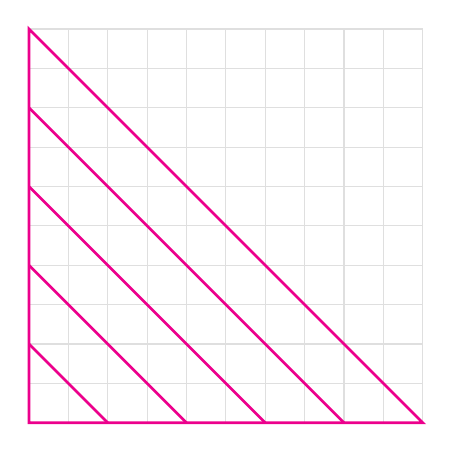
\begin{tikzpicture}
% Draw the blue grid
\draw[lightgray!50, step=0.5] (0,0) grid (5,5);

% Draw the magenta triangular pattern
\draw[magenta, line width=1pt] 
    (0,0) -- (0,5) -- (5,0) -- cycle;

% Draw the internal grid lines
\draw[magenta, line width=1pt] (0,1) -- (1,0);
\draw[magenta, line width=1pt] (0,2) -- (2,0);
\draw[magenta, line width=1pt] (0,3) -- (3,0);
\draw[magenta, line width=1pt] (0,4) -- (4,0);
\end{tikzpicture}
\end{minipage}

\end{example}

\begin{example}
若P为以原点为顶点,第一象限内的单位正方形,则
\begin{align*}
        &L_p(1)=4, \\
        &L_p(2)=9, \\
        &\vdots \\
        &L_p(n)=(n+1)^2=n^2+2n+1
    \end{align*}

\end{example}

观察上述两个例子,可以发现$L_p(n)$总可以写成关于$n$的多项式,且最高次等于该多胞体的维数。一般的,我们有以下定理:
\begin{theoreminner}[Ehrhart] 
对任意$d$维格点多胞体 $P$,
\begin{align}
L_p(n)=a_dn^d+a_{d-1}n^{d-1}+\cdots+a_1n+a_0,
\label{Ehrhart-polynomial}
\end{align}
其中$a_i\in\mathbb{Z}$。
\end{theoreminner}
定理中的$L_p(n)$ 称为多胞体 $P$ 的 $\textbf{Ehrhart 多项式}$, 系数$a_d, a_{d-1},\cdots,a_0$ 为多胞体$P$ 的 $\textbf{Ehrhart 系数}$。
关于Ehrhart 系数有结论如下:
\begin{align*}
&1.\ a_d=vol(P)\quad(P\text{的体积}),\\
&2.\ a_{d-1}=\text{facet的标准化体积总和的一半},\\
&3.\ a_0=1.
\end{align*}

\begin{remark}
    除了以上Ehrhart系数,其它系数的正性和多胞体本身的性质密切相关,具体可查看刘拂老师的文章\cite{FL19}。
\end{remark}
\begin{remark}
    Ehrhart多项式是对格点多胞体扩张(或缩小所在的格)之后格点数的计数,当取极限时格点数即是多胞体的体积。因此,Ehrhart多项式可以看作是格点多胞体的\textbf{离散体积},而这个离散体积作为一种 valuation,它恰好可以表为多项式。经典的 Hadwiger 定理刻画了 valuation 所形成的向量空间的基,在离散情形中也有类似结论,此处不详述。
\end{remark}


% \section{s-lecture hall polytope}
% 待更新,详情见陈端宇。


\section{Ehrhart 级数}

\begin{definition}
    给定一个格点多胞体 $ P \subseteq \mathbb{Z}^d $,$ P $ 的 Ehrhart 级数定义为
\begin{align*}
 \text{Ehr}_P(z) := \sum L_P(n) z^n
\end{align*}
其中 $ L_P(n) $ 为 P 的 Ehrhart 多项式。
\end{definition}\label{Ehrhart1}


\begin{example}
    令 $ P = \Delta_{d-1}:= \text{conv}\{e_i : i \in [d]\}$。

1.对于$\Delta_0$,$\operatorname{Ehr}_{\Delta_0}(z) = \sum_{n \geq 0} L_{\Delta_0}(n) z^n = \sum_{n \geq 0} z^n = \frac{1}{1-z}$.

% 插入图片
\begin{figure}[H] % [H] 表示强制当前位置
    \centering
    \includegraphics[width=0.5\textwidth]{image1.png} % 替换 "image.png" 为你的图片文件名
    \caption{零维单形扩张图} % 图片标题
    \label{fig:my_image} % 图片标签,用于引用
\end{figure}


2.对于$\Delta_1$,$\operatorname{Ehr}_{\Delta_1}(z) = \sum_{n \geq 0} L_{\Delta_1}(n) z^n = 1 + 2z + 3z^2 + \cdots = \frac{1}{(1-z)^2}$.

% 插入图片
\begin{figure}[H] % [H] 表示强制当前位置
    \centering
    \includegraphics[width=0.5\textwidth]{image2.png} % 替换 "image.png" 为你的图片文件名
    \caption{一维单形扩张图} % 图片标题
    \label{fig:my_image} % 图片标签,用于引用
\end{figure}



3.对于$\Delta_2$,$\operatorname{Ehr}_{\Delta_2}(z) =\sum_{n \geq 0} L_{\Delta_2}(n) z^n = \sum_{n \geq 0} \binom{n+1}{2} z^n = \frac{1}{(1-z)^3}$.

% 插入图片
\begin{figure}[H] % [H] 表示强制当前位置
    \centering
    \includegraphics[width=0.5\textwidth]{image3.png} % 替换 "image.png" 为你的图片文件名
    \caption{二维单形扩张图} % 图片标题
    \label{fig:my_image} % 图片标签,用于引用
\end{figure}



4.对于$\Delta_d$,$\operatorname{Ehr}_{\Delta_d}(z) = \sum_{n \geq 0} \binom{n+d}{d} z^n = \frac{1}{(1-z)^{d+1}}$.

\end{example}\label{Ehrhart1}

\begin{remark}
    思考:当 $ P = \Delta_{d-1}$时,其生成函数写成有理函数之后,分子也就是等式右边为什么恒为 1?
\end{remark}


\begin{example}
    令 $ P = \square_{d}:= \left\{(x_1, x_2, \ldots, x_d) \in \mathbb{R}^d : 0 \leq x_k \leq 1 , k \in [d] \right\}.$

1,对于$\square_2$,$L_{\square_2}(n) = (n+1)^2 $,

\begin{minipage}{0.5\textwidth}
    \begin{align*}
   \operatorname{Ehr}_{\square_2}(z) 
   &= \sum_{n \geq 0} L_{\square_2}(n) z^n \\
   &= \sum_{n \geq 0} (n+1)^2 z^n \\
   &= \frac{\sum_{k=1}^d A(2, k) z^{k-1}}{(1 - z)^{3}}.
    \end{align*}
\end{minipage}
\begin{minipage}{0.5\textwidth}
    % 插入图片
\begin{figure}[H] % [H] 表示强制当前位置
    \centering
    \includegraphics[width=0.8\textwidth]{image4.png} % 替换 "image.png" 为你的图片文件名
    \caption{$\square_2$扩张图} % 图片标题
    \label{fig:my_image} % 图片标签,用于引用
\end{figure}
\end{minipage}


2,对于$\square_d$,$ L_{\square_d}(n) = (n+1)^d $,
\begin{align*}
   \operatorname{Ehr}_{\square_d}(z) &= \sum_{n \geq 0} L_{\square_d}(n) z^n \\
   &= \sum_{n \geq 0} (n+1)^d z^n \\
   &= \frac{\sum_{k=1}^d A(d, k) z^{k-1}}{(1 - z)^{d+1}}.
\end{align*}

\end{example}\label{Ehrhart2}


\section{Coning 技巧与 $h^*$ 多项式}

对于单形而言,其 Ehrhart 级数是将每一层格点的总数作为系数;现在我们将其一般化,对于一个一般的格点多胞体,我们将其嵌入到更高一维,即在新构造的锥(cone)下计数格点数。这是处理 Ehrhart 多项式与级数的一种非常核心的技巧,暂称之为\textbf{Coning 技巧}。

\begin{definition}
    我们考虑一个格点多胞体 $\mathcal{P}$,其顶点为 $\mathbf{v}_1, \mathbf{v}_2, \ldots, \mathbf{v}_n \in \mathbb{Z}^d$。我们将这些顶点提升到 $\mathbb{R}^{d+1}$ 中,即通过添加一个 1 作为它们的最后一个坐标。即如果令
$$
\mathbf{w}_1 = (\mathbf{v}_1, 1), \ \mathbf{w}_2 = (\mathbf{v}_2, 1), \ \ldots, \ \mathbf{w}_n = (\mathbf{v}_n, 1).
$$
则
$$
\text{cone}(\mathcal{P}) = \left\{\lambda_1 \mathbf{w}_1 + \lambda_2 \mathbf{w}_2 + \cdots + \lambda_n \mathbf{w}_n : \lambda_1, \lambda_2, \ldots, \lambda_n \geq 0\right\} \subset \mathbb{R}^{d+1}.
$$
\end{definition}\label{coning1}
\begin{example}
    考虑下面这个由二维上升到三维的格点多胞体的例子。

令$
P := \Delta_1 \subset \mathbb{R}^2
\hookrightarrow \mathbb{R}^3
$,则有:

$$
P := \text{conv}\left\{ e_1 = \begin{pmatrix} 0 \\ 1 \end{pmatrix}, e_2 = \begin{pmatrix} 1 \\ 0 \end{pmatrix} \right\} \hookrightarrow \mathbb{R}\left\{ e'_1 = \begin{pmatrix} 1 \\ 0 \\ 0 \end{pmatrix}, e'_2 = \begin{pmatrix} 0 \\ 1 \\ 0 \end{pmatrix} \right\}
$$


% 插入图片
\begin{figure}[H] % [H] 表示强制当前位置
    \centering
    \includegraphics[width=1.0\textwidth]{image5.png} % 替换 "image.png" 为你的图片文件名
    \caption{${R}^2 \hookrightarrow \mathbb {R}^3$嵌入图} % 图片标题
    \label{fig:my_image} % 图片标签,用于引用
\end{figure}
\end{example} 

\begin{remark}
    将由此形成的锥里的每个格点对应单项式,我们发现所有的单项式可以构成一个半群代数,即$\mathbb{R}[\mathcal{P}] := \mathbb{R}[\text{cone}(\mathcal{P})]$。
\end{remark}

通过构造锥,我们将原来的格点多胞体的每个扩张的“备份”嵌入到了更高一维的相应高度,反过来,通过用超平面“切割”这个锥我们能完整复原原来的格点多胞体及其扩张。此时,格点多胞体的 Ehrhart 级数实际是对整个锥的计数,从代数的角度看它是半群代数的生成函数。

在上述定义下,由格点多胞体的 Ehrhart 级数所引出的$h^*$-多项式是研究的关键。

\begin{definition}
    假设 $P$ 是一个格点多胞体,\text{dim}P = d。P 的 $h^*$-多项式定义为:
\begin{align*}
    \operatorname{Ehr}_P(z) 
    &= 1 + \sum_{t \geq 1} L_P(t) z^t \\
    &:= \frac{h^*(z)}{(1-z)^{d+1}} \\
    &=\frac{h_d^* z^d + h_{d-1}^* z^{d-1} + \cdots + h_1^* z + h_0^*}{(1 - z)^{d+1}},
\end{align*}
\end{definition}

\maketitle
	\section{单纯复形与Stanley-Reisner环}
	\subsection{集合与子集}
	集合$$E=\{x_1,x_2,\dots,x_n\}$$简记为$$[n]:=\{1,2,\dots,n\}.$$
	
	\begin{definition}
		设集合$I\subset E$,$I$的特征函数定义为:$$\delta_I:E\to \{0,1\}$$其中
		$$\delta_I(i)=
		\begin{cases}
			1,& \mbox{若}i\in I,\\
			0,& \mbox{若}i\notin I.
		\end{cases}$$
	\end{definition}
	
	可以用单项式$\prod_{i\in I}x_i$或特征向量$v_I=(\delta_I(1),\delta_I(2),\dots, \delta_I(n))$表示$I$. 
	
	\begin{example}
		$E=\{1,2,3,4\}, I=\{1,4\}$可表示为$x_1x_4$或$v_I=(1,0,0,1).$
	\end{example}
	
	\begin{definition}
		若$I\subset E$且$|I|=k$, 则称$I$为$E$的$k$子集.
	\end{definition}

\subsection{重集}
为表述方便, 接下来默认$E=[n]$. 

\begin{definition}
	称$M=(E,\delta_E)$为重集, 若
		$$\delta_E(i)=
	\begin{cases}
		k_i,& \mbox{若}i\in E,\\
		0,& \mbox{若}i\notin E.
	\end{cases}$$
	其中$k_i\in \mathbb{Z}_{>0}$为$E$中$i$的重数.
	
	称$$S=\{i\in E | \delta_E(i)\neq 0\}$$为重集$M$的支撑集, 记$supp(M)=S$. 
\end{definition}

	\begin{example}
		设$E=\{1,2,3,4\}$, 且
		$$\delta_E(1)=2,\quad \delta_E(2)=2, \quad \delta_E(3)=1, \quad \delta_E(4)=0.$$
		则重集可表示为$M=\{1,1,2,2,3\}$, 且$supp(M)=\{1,2,3\}$
	\end{example}
	\begin{remark}
		子重集是指重集的子集, $k$子重集是指基数为$k$的子重集. 
	\end{remark}
	对于给定的集合$I\subset E=[n]$, 如何表示以$I$为支撑集的$k$子重集?
	\begin{example}
		设$I=\{1,3\}$, $|M|=4$. 则
		$$\{M | supp(M)=I, |M|=4\}=\{\{1,1,1,3\}, \{1,1,3,3\}, \{1,3,3,3\}\}.$$
	\end{example}
	
	\begin{lemma}
		设$I\subset E=[n]$, 且$|I|=m$. 记$X=\{M | supp(M)=I, |M|=k\}$, $Y=\{(z_1,z_2,\dots,z_m)\in \mathbb{Z}^m_{\geq 1} | \sum_{i=1}^mz_i=k\}$. 则$X$和$Y$之间存在一一映射. 
	\end{lemma}
	
	\begin{example}
		设$I=\{1,3,4\}$, $|M|=5$. 则
		$$M=\{t_1,t_2,t_3,t_4,t_5\}=\{\{1^{a_1},3^{a_2},4^{a_3}\} | a_1+a_2+a_3=5\}.$$ 
	\end{example}
	
	\begin{corollary}
		设$I\subset E=[n]$, 且$|I|=m$. 则$\# \{M | supp(M)=I, |M|=k\}=\binom{k-1}{m-1}.$
	\end{corollary}
	
	\subsection{梯度结构}
	
	$E$的子集可以通过$rank$函数生成一个有限梯度$Boolean\ lattic\ B_n$:
	$$rk: 2^E\to \mathbb{Z}_{\geq 0},\ I\mapsto |I|.$$
	
\begin{example}
	设$E=[3]$. 可得到$B_3$对应的哈斯图: 
		\vspace{-0.4cm} %调整图片与上文的垂直距离
		
%插入图片
\begin{figure}[H]
	\centering	
    \includegraphics[width=0.7\textwidth]{Boolean lattic B_3}
	\caption{$Boolean\ lattic\ B_3$}% 图片标题
\end{figure}
\end{example}
	
	$Boolean\ lattic\ B_n$的生成函数: 
	$$F(x_1,x_2,\dots,x_n)=1+\sum_{i=1}^nx_i+\sum_{1\leq i<j\leq n}x_ix_j+\cdots+x_1x_2\cdots x_n=\prod_{i=1}^n(1+x_i).$$
	令$x_1=x_2=\cdots=x_n=x$, 可得到: 
	$$F(x,x,\dots,x)=(1+x)^n :=\binom{n}{0}+\binom{n}{1}x+\binom{n}{2}x^2+\cdots+\binom{n}{n}x^n.$$
	同时得到了二项式系数的定义. 
	
	\begin{definition}
		集合$[n]$的$k$子集个数为$\binom{n}{k}$.
	\end{definition}
	
	\begin{remark}
		向量$(\binom{n}{0},\binom{n}{1},\binom{n}{2},\cdots,\binom{n}{n})$是$Boolean\ lattic\ B_n$(单纯复形$simplicial\ complex$)的$rank$向量($face$向量).
	\end{remark}
	
	所有子重集构成梯度晶格$L^{\infty}$. $Boolean\ lattic\ L^{\infty}$的生成函数为: 
	$$F(x_1,x_2,\dots,x_n)=1+\sum_{i=1}^{\infty}x_i+\sum_{i\leq j}x_ix_j+\cdots=\prod_{i=1}^n(1+x_i+x_i^2+\cdots)=\prod_{i=1}^n\frac{1}{1-x_i}.$$
	令$x_1=x_2=\cdots=x_n=x$, 可得到: 
	$$F(x, x, \dots, x) = \frac{1}{(1-x)^n} :=
    \left(\!\!{n\choose 0}\!\!\right) +\left(\!\!{n\choose 1}\!\!\right)x +\left(\!\!{n\choose 2}\!\!\right)x^2 + \dots 
    + \left(\!\!{n\choose n}\!\!\right)x^n +\dots.$$
	\begin{definition}
		集合$[n]$的$k$子重集个数为 $\left(\!\!{n\choose k}\!\!\right)=\binom{n+k-1}{k}$.
	\end{definition}
	
	\subsection{Down-closed性质}
	向下封闭$(deown-closed)$意味着: 如果$S\in \Delta$, 那么$S$的所有子集也必须属于$\Delta$. 
		\vspace{-0.4cm} %调整图片与上文的垂直距离
	
%插入图片
\begin{figure}[H]
	\centering
	\includegraphics[width=0.3\textwidth]{Boolean lattic B_3截断}
	\caption{$Boolean\ lattic\ B_3$截断}% 图片标题
\end{figure}

\subsection{单纯复形$Simplicial\ complex$}
	\begin{definition}
		一个单纯复形$\Delta$是一个向下封闭$(down-closed)$的子集族, 它是有限集合$[n]$(称为基集$ground\ set$)的子集的集合. 
	\end{definition}

		单纯复形的面$(face)$可理解为任何维度的子单纯形, 包括顶点、边、三角形等. 例如一个三角形(2维单纯形)的面包括它的三条边(1维单纯形)和三个顶点(0维单纯形). 对于$(facet)$, 可理解为在单纯复形中维数最大的单纯形, 或者是不被其他单纯形包含的单纯形. 

%插入图片
\begin{figure}[H]
	\centering 
	\begin{minipage}[b]{0.45\textwidth}
	\centering
        \includegraphics[width=0.7\textwidth]{facet举例}% 图片标题
		\caption{$facet$举例}
	\end{minipage}
	\begin{minipage}[b]{0.45\textwidth}
	\centering
		\includegraphics[width=1.2\textwidth]{face lattice}
		\caption{$face\ lattice$}% 图片标题
	\end{minipage}
\end{figure}
	
	\begin{definition}
		设$\tau \in\Delta$为一个$face$. 则$dim(\tau)=|\tau|-1$, $dim(\Delta)=\max\{dim(\tau):\tau $是一个$face\}$=$\max\{dim(\tau):\tau $是一个$facet\}$. 
	\end{definition}
	
	\subsection{Stanley-Reisner环}
	对于$[n]$上的一个$d$维单纯复形$\Delta$, 定义$face$向量$f=(f_{-1},f_0,f_1,\cdots,f_{d-1})$. 
		\vspace{-0.4cm} %调整图片与上文的垂直距离
%插入图片	
\begin{figure}[H]
	\centering
		\includegraphics[width=0.7\textwidth]{[4]上的2维单纯复形}
		\caption{$[4]$上的2维单纯复形}% 图片标题
		\label{Simplicial complex of 4} % 图片标签,用于引用
\end{figure}
	
\begin{definition}
		设$\mathbb{K}$是作为系数的交换环, 给定任何一个顶点集的单纯复形$\Delta$, $\Delta$关于$\mathbb{K}$的$Stanley-Reisner$环是指: 
		$$\mathbb{K}[\Delta]=\mathbb{K}[x_1, x_2, \cdots, x_n]/I_{\Delta}$$
		其中$I_{\Delta}$是由所有不属于$\Delta$的单形所对应的单项式生成的理想, 也称为$Stanley-Reisner$理想, 即$I_{\Delta}=<x_{\tau}: \tau \notin \Delta>$. 
\end{definition}
	例如, 图$\ref{Simplicial complex of 4}$所对应的$Stanley-Reisner$理想为$I_{\Delta}=<x_1x_4, x_2x_4, x_3x_4, \cdots>$, 相应的$Stanley-Reisner$环为$\mathbb{K}[\Delta]=\mathbb{K}[x_1,x_2,x_3,x_4]/I_{ \Delta}$.
	
	\begin{proposition}
		作为$\mathbb{K}$上的向量空间, $\Delta$的$Stanley-Reisner$环有直和分解: 
		$$\mathbb{K}=\oplus_{i=0}\mathbb{K}[\Delta]_i.$$
	\end{proposition}
	
	
\noindent
	\begin{minipage}[b]{0.6\linewidth}
		\centering
		\includegraphics[width=0.9\textwidth]{pic6}
	\end{minipage}
	\hfill
\begin{minipage}[b]{0.4\linewidth}
	\begin{align*}
		\mathbb{K}[\Delta]_0&:\ 1\\
		\mathbb{K}[\Delta]_1&:\ x_1,x_2,x_3\\
		\mathbb{K}[\Delta]_2&:\ x_1^2,x_1x_2,x_1x_3,x_2^2,x_2x_3,x_3^2\\
		\mathbb{K}[\Delta]_3&:\ x_1^3,\cdots,\widehat{x_1x_2x_3},\cdots
	\end{align*}
\end{minipage}

\section{Stanley-Reisner环}

\subsection{Epi-Mono mapping}
\begin{definition}
 如果 $P, Q$ 是偏序集,那么 $f: P \to Q$ 称为是\textbf{保序的}或\textbf{单调的},如果
$ x < y \implies f(x) < f(y). $
$f: P \to Q$ 称为(偏序集间的)\textbf{同构},如果 $f$ 是双射,并且 $f$ 和 $f^{-1}$ 都是保序映射。
\end{definition}\label{Ehrhart1}

令$[n] = \{1, 2, \ldots, n\}$, $I \subseteq [n]$,$|I| = m$.
那么我们有一下两个结论\\
$\bullet$保序的单射 $\iota: I \rightarrow [n]$的个数为:$\binom{n}{m}$,\\
$\bullet$ 保序的满射 $\pi: [n] \rightarrow I$的个数为:$\binom{n-1}{m-1}。 $  

\begin{example}
设 $ n = 5 $,且 $ I = \{2, 4\} $。\\
所有保序的单射的个数为:$\binom{5}{2} = 10。$\\
所有保序的满射的个数为:$\binom{4}{1} = 4。$
\end{example}

\subsection{Simplicial complex and multicomplex}
Simplicial Complex(单纯复形) 是拓扑学和组合数学中的一个重要概念,用于描述空间的离散结构。它由点、线段、三角形、四面体等更高维的“单纯形”组成,并且满足一定的组合性质。

\begin{definition}
一个单纯复形(也可简称复形 complex) $\mathcal{K}$ 是单纯形的集合,且满足:
\begin{enumerate}
    \item 若单纯形属于 $\mathcal{K}$,则其任意面都属于 $\mathcal{K}$,
    \item 若 $\sigma_1, \sigma_2$ 为 $\mathcal{K}$ 中的两个单纯形,则 $\sigma_1 \cap \sigma_2$ 是空集或者是 $\sigma_1, \sigma_2$ 共有的一个面。
\end{enumerate}
\end{definition}
简而言之,单纯复形就是向下封闭的集合的子集族。\\
令 $\Delta$ 是顶点集 $V = \{x_1, \ldots, x_n\}$ 上的一个有限单纯复形。这意味着 $\Delta$ 是 $V$ 的子集集合,使得如果 $F \subseteq G \in \Delta$,则 $F \in \Delta$,且对于所有 $x_i \in V$,$\{x_i\} \in \Delta$。$\Delta$ 的元素称为面(faces)。如果 $F \in \Delta$,则定义 $\dim F := |F| - 1$,并定义 $\dim \Delta := \max_{F \in \Delta} (\dim F)$。令 $d = \dim \Delta + 1$。给定任意域 $k$,我们现在定义 $\Delta$ 的面环(face ring)或斯坦利-赖斯纳环(Stanley-Reisner ring),记作 $k[\Delta]$。

\begin{definition}
$k[\Delta] = k[x_1, \ldots, x_n]/I_\Delta$,其中
$I_\Delta = \{x_{i_1} x_{i_2} \cdots x_{i_r} \mid i_1 < i_2 < \cdots < i_r,\quad \{x_{i_1}, x_{i_2}, \ldots, x_{i_r}\} \notin \Delta\}。$
\end{definition}

\begin{theoreminner}
$ \dim k[\Delta] = 1 + \dim \Delta = d。 $
\end{theoreminner}

\begin{theoreminner}
定义 $\deg x_i = 1$。那么
\begin{align}
H(k[\Delta], m) = \begin{cases} 
1, & m = 0 \\
\sum _{i=0}^{d-1}f_i \binom{m-1}{i}, & m > 0 
\end{cases}
\end{align}
等价地
\begin{align}
F(k[\Delta], \lambda) = \sum_{i=-1}^{d-1} \frac{f_i \lambda^{i+1}}{(1 - \lambda)^{i+1}}。
\end{align}
\end{theoreminner}


\begin{remark}
表达式 $\sum f_i \binom{m-1}{i}$ 在 $m = 0$ 时给出 $\Delta$ 的欧拉特征。因此,$k[\Delta]$ 的 Hilbert 函数在 $\chi(\Delta) = 1$ 时没有异常值。为了证明上述定理,最简单的方法是先使用更精细的分级,然后再进行特化。定义 $k[\Delta]$ 的精细分级为 $\deg x_i = (0, \ldots, 0, 1, 0, \ldots, 0) \in \mathbb{Z}^n$,其中 $i$ 是单位坐标向量。令 $x_1^{a_1} x_2^{a_2} \cdots x_n^{a_n} = \{x_i \mid a_i > 0\}$。显然,所有形如 $u = x_1^{a_1} x_2^{a_2} \cdots x_n^{a_n}$ 且 $u \in \Delta$ 的单式 $u$ 形成 $k[\Delta]$ 的 $k$-基。通过计算这些单式的支撑 $F \in \Delta$,我们得到精细分级的 Hilbert 系列的以下表达式:
\begin{align*}
 F(k[\Delta], \lambda) = \sum_{F \in \Delta} \prod_{x_i \in F} \frac{\lambda_i}{1 - \lambda_i}。
\end{align*}
\end{remark}

\begin{definition}
$(d-1)$维单纯复形的$f$-向量就是它的各维面的个数$f=(f_{-0}, f_{-1}, \cdots, f_{-(d-1)})$,$f_{-0}$就是其顶点数,$f_{-1}$就是边的个数,$\cdots$,$f_{-(d-1)}$就是其极大面积的个数。
\end{definition}

\begin{definition}
$\Delta$的Euler数定义为$e(\Delta)=f_{-0}-f_{-1}+f_{-2}\cdots+(-1)^{(d-1)}f_{-(d-1)}$
\end{definition}

由此可以计算$k[\Delta]$的($Z^n$分次的)Hilbert多项式
\begin{align*}
H_k[\Delta](t)& = \sum _{F \in \Delta} \sum_{a \in N^n, \text{supp}(a)=F} t^a\\
&=\sum_{F \in \Delta}\prod _{v_i \in F} \frac{t_i}{(1-t_i)}\\
&= \sum_{i=0}^{d-1} f_{-i} \frac{t^{i+1}}{(1-t)^{i+1}}。
\end{align*}

\begin{definition}
对于Stanley-Reisner环,我们有所谓的$h$-向量,它是通过其Hilbert多项式定义如下:
\begin{align*}
H_k[\Delta](t) = h_0 + h_1 t + \cdots + \frac{t^d}{(1-t)^d}。
\end{align*}
\end{definition}

比较上述两式,可以得到$f$-向量与$h$-向量之间的关系:
\begin{align*}
\sum h_i t^i = \sum_{i=0}^{d-1} f_{-(i-1)} \frac{t^i}{(1-t)^{d-i}}
\end{align*}
那么有
\begin{align*}
h_j = \sum _{i=0, \cdots, j} (-1)^{(j-i)} \binom{d-i}{j-i} f_{-(i-1)},
\end{align*}
和
\begin{align*}
f_{-(j-1)} = \sum _{i=0, \cdots, j} \binom{d-i}{j-i} h_i。
\end{align*}
特别地,我们可以得到几个容易计算的公式:
\begin{align*}
h_0 = 1, \quad h_1 = f_{-0} - d, \quad h_d = (-1)^{(d-1)} e(\Delta),
\end{align*}
以及
\begin{align*}
&\sum _{i=0, \cdots, d} h_i = f_{-(d-1)}。
\end{align*}
其中$e(\Delta) = e(\Delta)-1$是$\Delta$的约化Euler数,也可以视为$\Delta$的约化上同调的交错和。

\begin{theoreminner}
向量 $(f_0, f_1, \ldots, f_{d-1}) \in \mathbb{Z}^d$ 是某个 $(d-1)$-维单纯复形 $\Delta$ 的 $f$-向量当且仅当
\begin{align*}
0 < f_{i+1} \leq f_i^{(i+1)}, \quad 0 \leq i \leq d-2。
\end{align*}

\end{theoreminner}


与单纯复形一起,我们还需要多重复形的更一般概念。一个多重复形 $\Gamma$ 在顶点集 $V = \{x_1, \ldots, x_n\}$ 上是一个单式集合 $x_1^{a_1} \cdots x_n^{a_n}$,使得 $u \in \Gamma$,$v | u$ 意味着 $v \in \Gamma$。因此,单纯复形对应于平方自由单式的特殊情况。多重复形有时被拓扑学家称为“半单纯复形”。对于一个多重复形 $\Gamma$,令 $h_i := \# \{u \in \Gamma \mid \deg u = i\}$,并定义 $h$-向量 $h(\Gamma) = (h_0, h_1, \ldots)$。$h$-向量可能是无限的,如果 $\Gamma \neq \emptyset$,那么 $ h_0 = 1 $。

\begin{definition}
如果 $ h_i = 0 $ 对于 $ i > d $,我们也写 $ h(\Gamma) = (h_0, \ldots, h_d) $。序列 $ (h_0, h_1, \ldots) $ 是某个非空多重复形 $\Gamma$ 的 $ h $-向量,称为 $ M $-向量。
\end{definition}

\begin{theoreminner}
$ (h_0, h_1, \ldots) $ 是一个 $ M $-向量当且仅当 $ h_0 = 1 $ 并且 $ 0 \leq h_{i+1} \leq h_i^{(i)}, i \geq 1 $。
\end{theoreminner}

\subsection{Simplicial polytope}

\begin{definition}
在几何学中,一个单纯形(simplicial polytope)是一个三角形或四面体的概念向任意维度的推广。命名为单纯形是因为它表示任意已知维度中最简单的多面体 (polytope)。具体来说,一个$k$ 维单纯形就是一个$k$维多面体,即是其 $(k+1)$ 个顶点的凸包。
\end{definition}
\begin{example}
一个0维单纯形(0-dimensional)是一个点。\\
一个1维单纯形(1-dimensional)是一条线段。\\
一个2维单纯形(2-dimensional)是一个三角形。\\
一个3维单纯形(3-dimensional)是一个多面体。\\
一个4维单纯形(4-dimensional)是一个5点细胞体(5-cell)。
\end{example}

\begin{remark}
Polytope 是一种高维的几何对象,它是通过有限个平面切割空间而得到的一个有界集合。简单来说,它是一个在任意维度上都有明确边界的形状。在一维中,它是一条线段;在二维中,它是多边形;在三维中,它是多面体;在更高维度中,则是相应的高维形式。它的特点是有顶点、边、面等不同维度的“面”,这些面按照一定的规则组合在一起。\\
Simplicial complex 是由多个单纯形(如点、线段、三角形、四面体等)组成的结构,其中每一个单纯形的边界也是该结构的一部分,并且两个单纯形要么不相交,要么只在其公共面(可能是点)上相交。单纯复形可以用来构建更复杂的形状,不仅限于凸形或连通的空间,而且可以在任何维度上定义。\\
Simplicial polytope 是一种特殊的 polytope,它的所有面都是单纯形。换句话说,在 simplicial polytope 中,每个面(包括其自身)都可以被表示为一个单纯形。\\
polytope 是一个广泛的概念,适用于任意维度的有界几何对象;simplicial complex 是由单纯形组成的结构,可用于表示各种复杂形状;而 simplicial polytope 则是一种特殊类型的 polytope,其所有面都必须是单纯形。他们的关系如下图所示:

\begin{figure}[H] % [H] 表示强制当前位置
    \centering
    \includegraphics[width=0.5\textwidth]{关系图.png} % 替换 "image.png" 为你的图片文件名
    \caption{关系图} % 图片标题
    \label{fig:my_image} % 图片标签,用于引用
\end{figure}
\end{remark}


\subsection{Stanley-Reisner环}

\begin{definition}
设 $k$ 是作为系数的交换环,给定任何一个顶点集为 $\{v_1, \ldots, v_n\}$ 的单纯复形 $\Delta$,$\Delta$ 关于 $k$ 的 Stanley-Reisner 环是指商 $k$-代数:
$ k[\Delta] = k[x_1, \ldots, x_n] / I_\Delta $
其中 $I_\Delta$ 是由所有使得不属于 $\Delta$ 的单形 $\langle v_{i_1} \cdots v_{i_k} \rangle$ 所对应的单项式 $x_{i_1} \cdots x_{i_k}$ 生成的理想,也称为 Stanley-Reisner 理想。
即$ I_\Delta = [m; m \notin \Delta] $。
\end{definition}
把 $k[\Delta]$ 看作是由各维度上的向量空间组成的直和,则有:
$k[\Delta]=\bigoplus_{i=0}^{\infty} (k[\Delta])_i。$

\subsection{Hilbert 函数}
\begin{definition}
对于每个非负整数 $i$,定义 $k[\Delta]$ 的 Hilbert 函数 $h_{k[\Delta]}(i)$ 为:
$ h_{k[\Delta]}(i) = \dim_k ((k[\Delta])_i) $
这里 $(k[\Delta])_i$ 表示 $k[\Delta]$ 中次数为 $i$ 的部分。
\end{definition}

\section{h-vectors}
\subsection{$Hilbert$级数 }
先回顾前面的知识。\\
在$[n]$上给定一个单纯复形$\Delta$,假设$\Delta$的维数$dim \Delta =d-1$,那么对应的哈斯图($Hasse$)最上面一层代表$\Delta$极大面个数有$d$个。给定任意域 ${\mathbb{K}}$,则$\Delta$的面环(face ring)为$\mathbb{K}[\Delta] =\mathbb{K}[x_1, x_2, \ldots, x_n]/I_\Delta$,其中
$I_\Delta =\{x_{\tau}\ ,\tau \notin \Delta\}$为一个理想。
\begin{lemma}
若$f: \mathbb{N} \rightarrow \mathbb{C}$,$d \in \mathbb{N}$,则有
\begin{align}
\sum_{n=0}^{\infty}f(n)x^{n}=\frac{P(x)}{(1-x)^d}.
\label{eq1}
\end{align}
这里,$P(x) \in \mathbb{C}[x]$,$deg(P) \leq d$。
\end{lemma}

\begin{df}
若 $\Delta$ 的面环 $\mathbb{K}[\Delta]$ 存在,那么它的Hilbert 级数为
\begin{align}
F(\mathbb{K}[\Delta],z)&=\sum_{i=0}^{\infty}(dim\mathbb{K}[\Delta]_{i})z^{i}\nonumber \\[0.5ex]
&=\sum_{i=0}^{\infty}M_{i}z^{i}\nonumber \\[0.5ex]
&=\frac{h_{0}+h_{1}+h_{2}z^2+...+h_{d}z^{d}}{(1-z)^d}.\label{eq2}
\end{align}
其中(Stanley),
\begin{align}
M_{i} = \begin{cases}
1, & m = 0 \\
\sum_{i=0}^{d-1} f_j \binom{i-1}{j}, & m > 0.
\end{cases} \label{eq3}
\end{align}
这里\,$f_{j}$ 是$\Delta$中$j$-维单形的数量。
\end{df}\label{Ehrhart1}

可以发现,为了得到定义\,(\ref{eq2}) 式右边,首先要得到单纯复形$\Delta$每一层的维数公式\,$M_{i}$,再由引理\,(\ref{eq1}) 式推导得到。\par
$M_{i}$ 的理解如之前所讲,对于如下图\ref{fig1}的一个$\Delta$,
\begin{figure}[H] % [H] 表示强制当前位置
\centering % 关键命令:使内容居中
    \includegraphics[width=1.2\textwidth]{tupianyi.png}
    \caption{由单纯复形张成的多重复形的例子}% 图片标题
    \label{fig1} % 图片标签,用于引用
\end{figure}
\noindent 所得到的多重复形正好是$Stanley-Reisner$ $ring$每一层向量空间的积。\par
多重复形(图\ref{fig1}右边)的第一层表示向量乘积$x_{1}$,$x_{2}$,$x_{3}$,第二层表示向量乘积 $x^{2}_{1}$,$x_{1}x_{2}$,$x_{1}x_{3}$,$x^{2}_{2}$,$x^{2}_{3}$。$Stanley$ 公式表示的是要数多重复形某一层到底有多少个元素,换言之,即要数某一层向量空间的积的个数,而多重复形的维数可以由它对应的单纯复形的面向量($face$ $vectors$)表示出来,这意味着,当从偏序集的角度来看时,图\ref{fig1}右边可以进行横向拆分(每一层如何由前一层生成)。综上所述,给定一个$\Delta$,构造出它的面向量,就可以得到其$Hilbert$级数。

\subsection{h-vectors }

如果不借助第一节所述分解机制,能否由定义直接得到\,$h-vectors$或者$Hilbert$ 多项式,也就是直接得到\,(\ref{eq2})式最右边的结果。
\begin{df}
将\,$h=(h_{0},h_{1},h_{2},...,h_{d})$ 称为单纯复形\,$\Delta$ 的\,$h-vector$。
\end{df}\label{Ehrhart2}
通过一个例子再次理解\,$h-vector$ 的含义。
\begin{example}
如图$\,\ref{fig2}$ 的 $\Delta$ \par
\begin{figure}[h]
\centering
  % Requires \usepackage{graphicx}
\includegraphics[width=1.2\textwidth]{tupianer.png}
\caption{单纯复形及其多重复形}
\label{fig2}
\end{figure}
\noindent $dim \mathbb{K}[\Delta]]_{i}$表示多重复形每一层向量空间积的个数。那么,它所对应的\,$Hilbert$ 级数为
\begin{align}
F(\mathbb{K}[\Delta],z)&=\sum_{i=0}^{\infty}(dim\mathbb{K}[\Delta]_{i})z^{i}\nonumber \\[0.5ex]
&=1 + 3z +6 z^{2} + 9 z^{3} + 12 z^{4}+... \nonumber \\[0.5ex]
&=\frac{h(z)}{(1-z)^2}. \label{eq4}
\end{align}
\end{example}
(\ref{eq4}) 式右边\,$\frac{h(z)}{(1-z)^2}$ 表示选不同面(face)张成的多重复形对应的生成函数。当遍历\,$\Delta$ 所有的面时,多重复形的纵向分解完成,得到完整的\,$Hilbert$ 级数。\\

\begin{example}
图$\,\ref{fig3}$ 中的的两条射线对应的生成函数可以写成
\begin{align}
1+x+x^2+x^3+x^4+...=\frac{1}{1-x},~~~~~~~
x^4+x^5+x^6+x^7+x^8+...=\frac{x^4}{1-x}
\label{eq5}
\end{align} 
\begin{figure}[h]
\centering
\includegraphics[width=0.3\textwidth]{tupiansi.png}
\caption{平面上射线的例子}
\label{fig3}
\end{figure}
\end{example}

(\ref{eq5}) 式分子部分的不同表示第二条射线与第一条射线相比向右平移了4个单位长度。类似地,在二维空间的也有相同的结,(\ref{eq4}) 式右边的理解也如此。

\begin{df}
对一个单纯复形$\Delta$,任选一个它的面$\sigma$,则$M_{\sigma}=\{\mu \mid support(\mu)=\sigma\}$.
\end{df}

如图\,\ref{fig2} 选\,$\sigma=13\in\Delta$,则\,$M_{\sigma}=\{13, 113, 133, 1113, 1133, 1333,...\}$。

\begin{theoreminner}
若$\sigma=\{i_{1},i_{2},i_{3},...,i_{s}\}\in \Delta$,$M_{\sigma}:=\{x_{\sigma}=x^{\alpha_{1}}_{i_{1}}x^{\alpha_{2}}_{i_{2}}x^{\alpha_{3}}_{i_{3}}...x^{\alpha_{s}}_{i_{s}}\mid\sigma\in\Delta,\alpha_{i}\in\mathbb{Z}_{>0}\}$,
则
\begin{align}
\sum_{\mu\in M_{\sigma}}z^{deg(\mu)}=\prod_{\pi_{j}\in\sigma}(\sum_{d_{j}=1}z^{\alpha_{j}})=\frac{z^{s}}{(1-z)^{s}},
\label{eq6}
\end{align}
遍历\,$\Delta$ 中所有的面
\begin{align}
F(\mathbb{K}[\Delta],z)&=\sum_{\sigma\in\Delta}\frac{z^{\mid\sigma\mid}}{(1-z)^{\mid\sigma\mid}} \label{eq7}\\
&=\sum_{i=0}^{d}f_{i-1}\frac{z^{i}}{(1-z)^{i}} \label{eq8}\\
&=\sum_{i=0}^{d}f_{i-1}\frac{z^{i}(1-z)^{d-i}}{(1-z)^{d}} \label{eq9}\\
&:=\frac{\sum_{i=0}^{d}h_{i}z^{i}}{(1-z)^{d}}.
\label{eq10}
\end{align}
\end{theoreminner}

(\ref{eq7}) 式是对\,$\Delta$ 面的加和,(\ref{eq8}) 式是对其多重复形维数的加和,(\ref{eq9}) 式为多重复形\,$d-1$ 的形式,(\ref{eq10}) 式明确了\,$h_{i}$ 和\,$h-vector$ 的关系,即
\begin{align}
\sum_{i=0}^{d}f_{i-1}z^{i}(1-z)^{d-i}&=f_{-1}(1-z)^{d}+f_{0}z(1-z)^{d-1}+...+f_{d-1}z^{d}\nonumber \\[0.5ex]
&=h_{0}+h_{1}z+...+h_{d}z^{d}. \label{eq11}
\end{align}

\subsection{Stanley's  trick }
介绍一种由\,$f$ 向量直接得到\,$h$向量的技巧。\\

\begin{df}
给一个\,$\Delta$,有\,$f={f_{0},f_{1},f_{2},...,f_{d-1}}$ 。\par
\begin{figure}[h]
\centering
\includegraphics[width=0.8\textwidth]{tupianwu.png}
\caption{Stanley's \,trick}
\label{fig4}
\end{figure}
\end{df}

将表格 \,\ref{fig4} 的左上角至右下角依次写\,$f$ 向量,右上角至左下角全部标为\,$1$,此后每一行的量由上一行与之相邻的右侧量与左侧量做减法得到,表格最底部的量即是\,$\Delta$ 对应的\,$h$ 向量。

从矩阵的角度来考虑\,$f$ 向量和\,$h$ 向量的关系。
\begin{theoreminner}
如果将\,$\Delta$ 对应的\,$f$ 和\,$h$ 向量按倒序写成列向量的形式,那么与定义等价的矩阵表达形式为
\begin{equation}  \label{eq3.12}
\left[
\begin{array}{cccccc} % 6列均居中对齐(c: center)
\binom{0}{0} & \binom{1}{0} & \binom{2}{0} & ... & \binom{d-1}{0} & \binom{d}{0} \\ % 第1行
\binom{0}{1} & \binom{1}{1} & \binom{2}{1} & ... & \binom{d-1}{1} & \binom{d}{1} \\ % 第2行
... & ... & ... & ... & ... & ... \\ % 第3行
\binom{0}{d-1} & ... & ... & ... & \binom{d-1}{d-1} & \binom{d}{d-1} \\ % 第3行
\binom{0}{d} & \binom{1}{d} & \binom{2}{d} & ... & \binom{d-1}{d} & \binom{d}{d}    % 第4行(最后一行不加\\)
\end{array}
\right]
\left[
\begin{array}{ccccc}
h_{d}\\
h_{d-1}\\
... \\
h_{1} \\
h_{0} \\
\end{array}
\right]=
\left[
\begin{array}{ccccc}
f_{d-1}\\
f_{d-2}\\
... \\
f_{0} \\
f_{-1} \\
\end{array}
\right],
\end{equation}
其中,二项式系数\,$\binom{i}{j}$,\,$0\leq i\leq d, 0\leq j\leq d$,分别为矩阵的列指标和行指标。将
\begin{equation}  \label{eq3.12}
M=\left[
\begin{array}{cccccc} % 6列均居中对齐(c: center)
\binom{0}{0} & \binom{1}{0} & \binom{2}{0} & ... & \binom{d-1}{0} & \binom{d}{0} \\ % 第1行
\binom{0}{1} & \binom{1}{1} & \binom{2}{1} & ... & \binom{d-1}{1} & \binom{d}{1} \\ % 第2行
... & ... & ... & ... & ... & ... \\ % 第3行
\binom{0}{d-1} & ... & ... & ... & \binom{d-1}{d-1} & \binom{d}{d-1} \\ % 第3行
\binom{0}{d} & \binom{1}{d} & \binom{2}{d} & ... & \binom{d-1}{d} & \binom{d}{d}    % 第4行(最后一行不加\\)
\end{array}
\right].
\end{equation}
称为由\,$h$ 向量到\,$f$ 向量的过渡矩阵。
\end{theoreminner}
注意,矩阵\,$M$ 与其过渡矩阵\,$M^{-1}$ 有相同的表达形式。尽管\,$h$ 向量和\,$f$ 向量可以相互推导,但在研究过程中,学者们更关注\,$h$ 向量。

\subsection{Dehn-Sommerville Relation }
\begin{df}
如果\,$\Delta$是一个单纯球体 (simplicial sphere),则
\begin{align}
h_{i}=h_{d-i}.
\label{eq14}
\end{align}
\end{df}

\begin{example}
$h_{0}=f_{-1}$,\par
$h_{d}=f_{d-1}-f_{d-2}+...+f_{-1}$,\par
由\,$h_{0}=h_{d}$,得到\,$f_{d-1}-f_{d-2}+...-f_{0}+(-1)^{d}f_{-1}=f_{-1}$,
整理得到欧拉示性数($Euler \,characteristic$),$\chi(\Delta)=f_{0}-f_{-1}+f_{2}+..+f_{d-1}=0$。
欧拉示性数描述了\,$f$ 向量的一个线性关系,而$\,h_{i}=h_{d-i}$ 描述了\,$\Delta$ 的$\frac{d}{2}$个线性关系。
\end{example}
\begin{df}
给定一个$\,\Delta$,则它对应的\,$g$ 向量为
\begin{align}
g_{i}=h_{i}-h_{i-1}.
\label{eq15}
\end{align}
\end{df}




\begin{thebibliography}{99}
\bibitem[AY21]{AY21} Adiprasito K, Yashfe G. The partition complex: an invitation to combinatorial. Surveys in combinatorics 2021. 2021 Jun 24;470:1.
\bibitem[FL19]{FL19} L. FU, On positivity of Ehrhart polynomials,  In: Barcelo, H., Karaali, G., Orellana, R. (eds) Recent Trends in Algebraic Combinatorics. Association for Women in Mathematics Series, vol 16. Springer, Cham, 2019.
\bibitem[BR15]{BR15} M. Beck, S. Robins, Computing the continuous discretely 2ed., Springer, New York, 2015.
\bibitem[Li25]{Li25} 李文威, 代数学讲义(网络版)
\bibitem[Li25]{Li25} 李文威, 代数学方法(卷一)(网络版)
\bibitem[Li25]{Li25} 李文威, 代数学方法(卷二)(网络版)
\bibitem[Li25]{Li25} 李文威, 代数学方法(卷二)(网络版)
\bibitem[Sta96]{Sta96}
R.P. Stanley, Combinatorics and Commutative Algebra,
2ed., Birkh\"auser,  Boston, 1996,53--67.
\bibitem[ZG12]{ZG12}
Ziegler, G$\ddot{u}$nter M. Lectures on polytopes. Vol. 152. Springer Scienc and Business Media, 2012.

\end{thebibliography}

% Appendix (if needed)
%\appendix
%%\chapter{附录A}
%这是附录的内容.  

\end{document}
